\documentclass{article}

% Required packages
\usepackage{graphicx}
\usepackage{tocloft}
\usepackage{float}
\usepackage{caption}
\captionsetup[figure]{skip=5pt}
 

% Required packages
\usepackage[a4paper, margin=2cm]{geometry}
\usepackage{graphicx}
\usepackage{tocloft}

% Custom command for adding images with caption
\newcommand{\myimage}[2]{%
  \begin{figure}[htbp]
    \centering
    \includegraphics[width=0.8\textwidth]{#1}
    \caption{#2}
    \label{fig:#1}
  \end{figure}%
}

% Customizing section and subsection appearance
\usepackage{titlesec}
\titleformat{\section}{\Large\bfseries}{\thesection}{1em}{}
\titleformat{\subsection}{\large\bfseries}{\thesubsection}{1em}{}

% Customizing table of contents appearance
\renewcommand{\cftsecfont}{\bfseries}
\renewcommand{\cftsubsecfont}{\normalfont}
\renewcommand{\cftsecpagefont}{\normalfont}
\renewcommand{\cftsubsecpagefont}{\normalfont}

% Customizing spacing between sections and figures
\usepackage{setspace}
\setlength{\cftbeforesecskip}{10pt}
\setlength{\cftbeforesubsecskip}{5pt}
\setlength{\intextsep}{10pt}
% Custom command for adding images with caption


\begin{document}




 %Title and table of contents
\title{Block1 Laborbericht W\_BWI\_D\_03}
\author{Ali Alkhiami}
\date{\today}
\maketitle
\tableofcontents
\newpage



% Section 1
\section{Übung1}
\subsection{Betroffener Geschäftsprozesse}
\begin{figure}[H]
\vspace{-10pt}
  \centering
  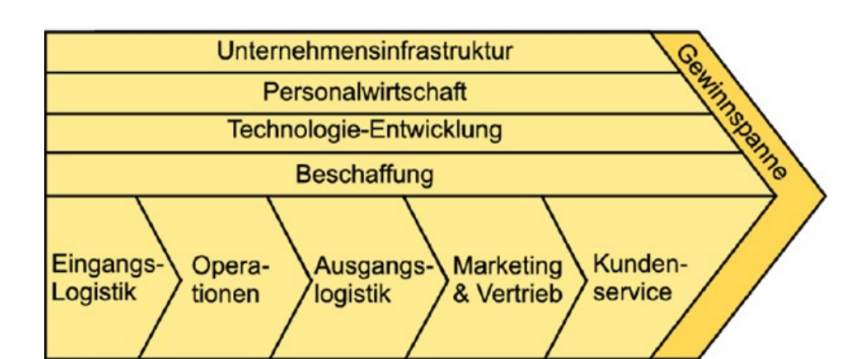
\includegraphics[width=0.8\textwidth]{land.png}
  \caption{von Benz }
  \label{fig:image}
\end{figure}



Wir befinden uns in der Materialbedarfsplanung und im Wareneingang, im Bezug auf die Prozesse im Buch von Benz.


\section{Erstellung eines Absatzplanes}
\subsection{Ziel: }
 nachdem wir  die Stammdaten und Arbeitsplatze/Pläne angelegt haben, wollen wir nun mit hilfe einer Prognose einen Absatzplan erstellen, die Prognose wurde erstellt basiert auf Historscher Werte, dann für die Absatzplan erstellen wir einen Produktiongrobplan und das soll als Produtionsprogramm übergeben werden.
 
 \subsection{Erstellung von F102}
wir wollen nun neuen FERT produkt anlegen und das aus F101 kopieren, um einen Produktgruppe erstellen zu können.
Dafür brauchen wir die Transiktion mm01 und die refrenz auf f101 um davon die Werte zu kopieren.
\begin{figure}[H]
\vspace{-10pt}
  \centering
  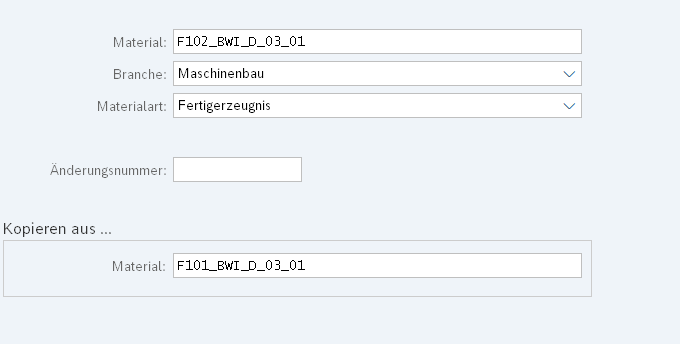
\includegraphics[width=0.8\textwidth]{f102.png}
  \caption{f102 anlegen}
  \label{fig:image}
\end{figure}
nun können wir die Produktgruppe für beide Matriallen anlegen, das machen wir mittels die Transiktion MC84
\begin{itemize}

\begin{figure}[H]
\vspace{-10pt}
  \centering
  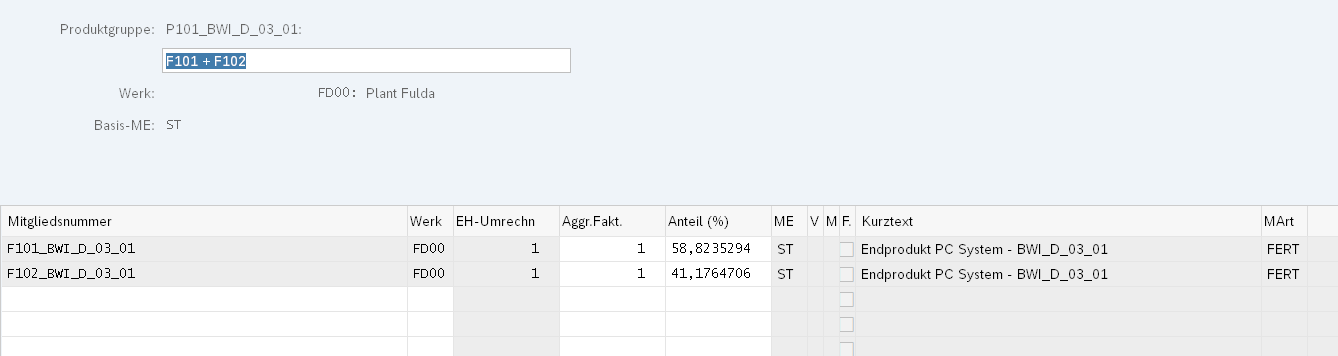
\includegraphics[width=0.8\textwidth]{p101.png}
  \caption{Produktgruppe anlegen }
  \label{fig:image}
\end{figure}
und können wir nun das Graphisch anzeigen lassen, man sieht dass die Materialien f101, f102 unter die Gruppe p101 sind 
\begin{figure}[H]
\vspace{-10pt}
  \centering
  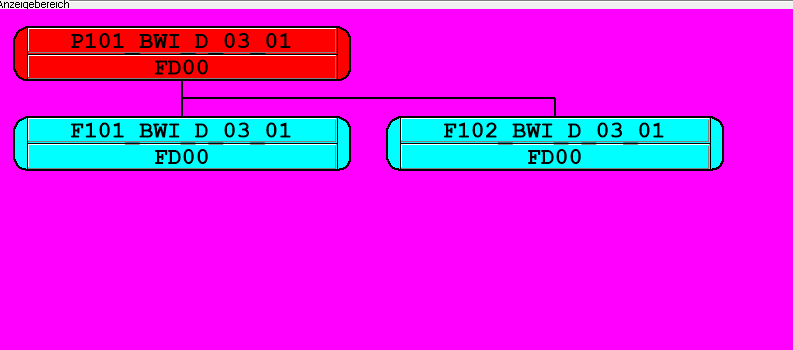
\includegraphics[width=0.8\textwidth]{gra.png}
  \caption{von Benz }
  \label{fig:image}
\end{figure}



\subsection{Prognose Sicht anlegen für f101 und f102}
MM01 um die neue Sicht anzulegen, dann habe ich die Prognosemodell auf Kostentmodell gesetzt

\begin{figure}[H]
\vspace{-10pt}
  \centering
  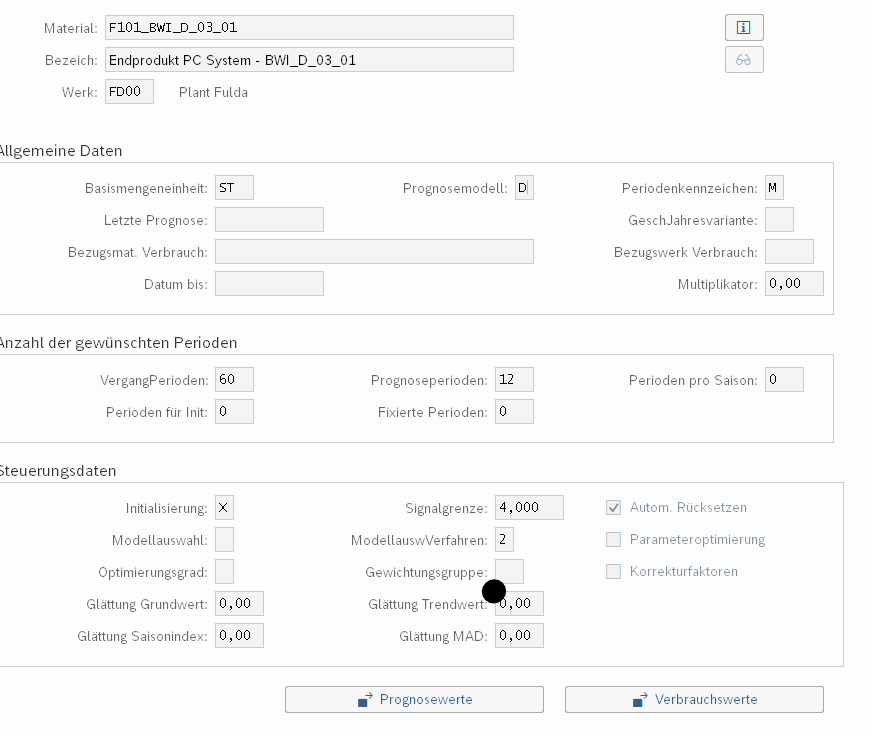
\includegraphics[width=0.8\textwidth]{kostenmodel.png}
  \caption{Prognose Sicht anlegen }
  \label{fig:image}
\end{figure}

in Prognose Sicht kann man die Historsche Werte pflegen.
\begin{figure}[H]
\vspace{-10pt}
  \centering
  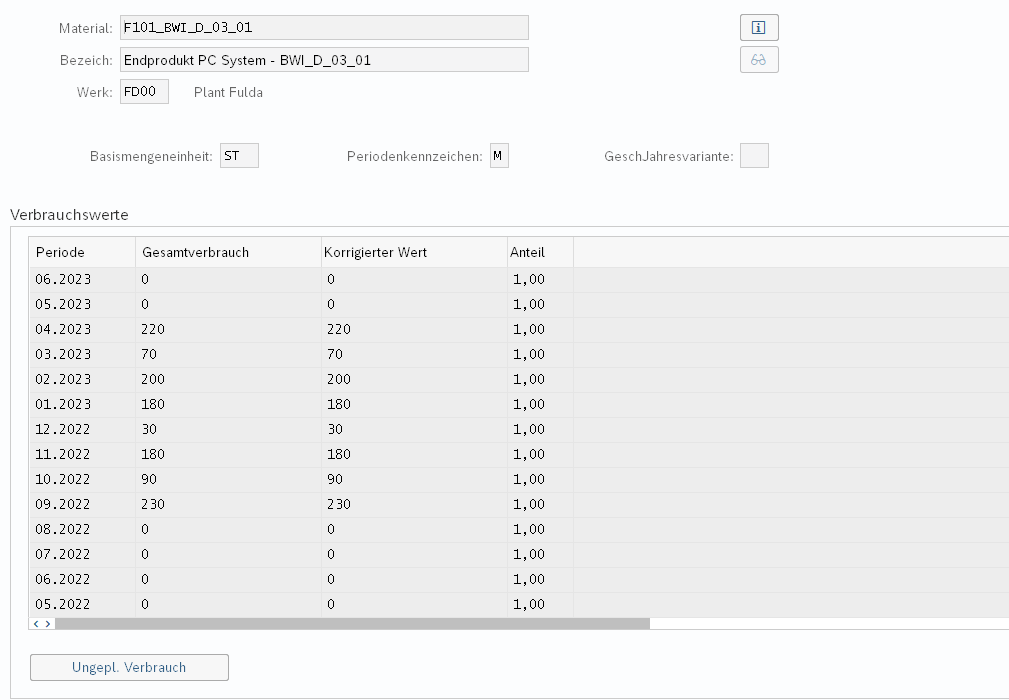
\includegraphics[width=0.8\textwidth]{wer.png}
  \caption{Historsche Werte pflegen }
  \label{fig:image}
\end{figure}


Dann steigen wir mit Transktion mc86 ein, um die Anteilsfaktoren aus die historische Werte der beiden Materialien richtig anzulegen.

\begin{figure}[H]
\vspace{-10pt}
  \centering
  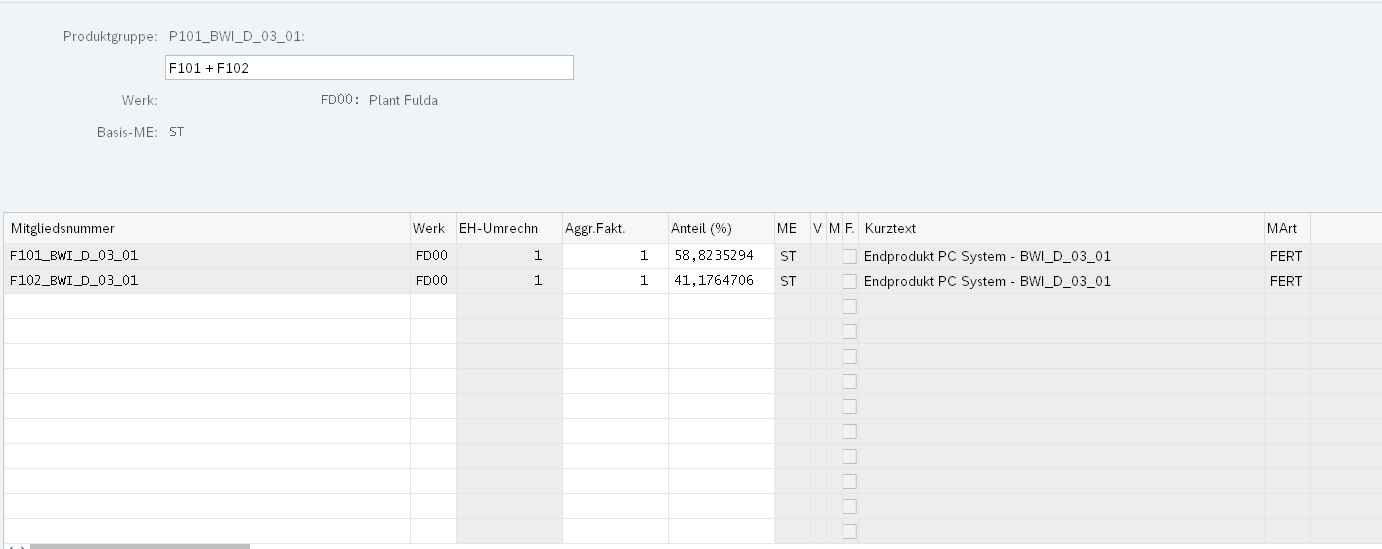
\includegraphics[width=0.8\textwidth]{anteil.png}
  \caption{Anteilsfaktoren }
  \label{fig:image}
\end{figure}




\item \textbf{bp:} Wir erfassen einen neuen Lieferanten mit verschiedenen Ansichten und pflegen die erforderlichen Informationen und Daten.
\item\textbf{MKVZ:} Anzeigen der Lieferanten.
\item\textbf{MM01:} Wir erstellen ein Material und geben verschiedene Ansichten ein. Die erforderlichen Ansichten hängen von der Art des Materials ab. Es ist wichtig, die obligatorischen Ansichten korrekt auszufüllen. Bei Bedarf können später weitere Ansichten hinzugefügt oder mit MM01 geändert werden.
\item\textbf{MM02:} Nachdem das Material erstellt wurde, können wir die Materialdaten mit MM02 ändern.
\item\textbf{MM03:} Mit MM03 können wir uns die erstellten Materialdaten anzeigen lassen.
\item\textbf{MM60:} Anzeigen einer Übersicht über Materialien.
\end{itemize}


\end{document}


